% !TeX TXS-program:compile = txs:///arara
% arara: pdflatex: {shell: yes, synctex: no, interaction: batchmode}
% arara: pdflatex: {shell: yes, synctex: no, interaction: batchmode} if found('log', '(undefined references|Please rerun|Rerun to get)')

\documentclass[a4paper]{article}
\usepackage[english]{babel}
\usepackage[utf8]{inputenc}
\usepackage[T1]{fontenc}
\usepackage{WriteOnGrid}
\usetikzlibrary{decorations.pathreplacing}
\usepackage{amsmath,amssymb}
\usepackage{fontawesome5}
\usepackage{enumitem}
\usepackage{frcursive}
\usepackage{lipsum}
\usepackage{tabularray}
\usepackage{fancyvrb}
\usepackage{fancyhdr}
\fancyhf{}
\renewcommand{\headrulewidth}{0pt}
\lfoot{\sffamily\small [WriteOnGrid]}
\cfoot{\sffamily\small - \thepage{} -}
\rfoot{\hyperlink{matoc}{\small\faArrowAltCircleUp[regular]}}

\usepackage{hologo}
\usepackage{xspace}
\newcommand\tikzlogo{Ti\textit{k}Z}
\newcommand\TeXLive{\hologo{TeX}Live\xspace}
\let\TikZ\tikzlogo
\newcommand\TableauDocumentation{%
	\begin{tblr}{width=\linewidth,colspec={X[c]X[c]X[c]X[c]X[c]X[c]},cells={font=\sffamily}}
		{\huge \LaTeX} & & & & &\\
		& {\huge \hologo{pdfLaTeX}} & & & & \\
		& & {\huge \hologo{LuaLaTeX}} & & & \\
		& & & {\huge \TikZ} & & \\
		& & & & {\huge \TeXLive} & \\
		& & & & & {\huge \hologo{MiKTeX}} \\
	\end{tblr}
}

\usepackage{hyperref}
\urlstyle{same}
\hypersetup{pdfborder=0 0 0}
\usepackage[margin=1.5cm]{geometry}
\setlength{\parindent}{0pt}
\definecolor{LightGray}{gray}{0.9}

\def\TPversion{0.1.7}
\def\TPdate{01/09/2024}

\usepackage[most]{tcolorbox}
\tcbuselibrary{minted}
\NewTCBListing{PresentationCode}{ O{blue} m }{%
	sharp corners=downhill,enhanced,arc=12pt,skin=bicolor,%
	colback=#1!1!white,colframe=#1!75!black,colbacklower=white,%
	attach boxed title to top right={yshift=-\tcboxedtitleheight},title=Code \LaTeX,%
	boxed title style={%
		colframe=#1!75!black,colback=#1!15!white,%
		,sharp corners=downhill,arc=12pt,%
	},%
	fonttitle=\color{#1!90!black}\itshape\ttfamily\footnotesize,%
	listing engine=minted,minted style=colorful,
	minted language=tex,minted options={tabsize=4,fontsize=\footnotesize,autogobble},
	#2
}

\newcommand\Cle[1]{{\bfseries\sffamily\textlangle #1\textrangle}}

\begin{document}

\pagestyle{fancy}

\thispagestyle{empty}

\vspace{2cm}

\begin{center}
	\begin{minipage}{0.75\linewidth}
	\begin{tcolorbox}[colframe=yellow,colback=yellow!15]
		\begin{center}
			\begin{tabular}{c}
				{\Huge \texttt{WriteOnGrid [en]}}\\
				\\
				{\LARGE To write on lines} \\
				{\LARGE of a grid.}
			\end{tabular}
			
			\medskip
			
			{\small \texttt{Version \TPversion{} -- \TPdate}}
		\end{center}
	\end{tcolorbox}
\end{minipage}
\end{center}

\vspace{0.5cm}

\begin{center}
	\begin{tabular}{c}
	\texttt{Cédric Pierquet}\\
	{\ttfamily c pierquet -- at -- outlook . fr}\\
	\texttt{\url{https://github.com/cpierquet/WriteOnGrid}}
\end{tabular}
\end{center}

\vspace{0.5cm}

{$\blacktriangleright$~~Some commands to create a grid (5x5 or Seyes or Ruled) and to write "on" the lines.}

\smallskip

{$\blacktriangleright$~~Possibility to personnalize size, margins, ...}

\vspace{1cm}

\begin{center}
	\begin{EnvGrid}[NumSquares=22x8]
	\WriteLine{my text on line 1\ldots}
	\WriteLine<center>{my centered text on line 2\ldots}
	\WriteLine<right>{my right-align text on ligne 3\ldots}
	\WriteLine[OffsetH=2]{my 2-squares shifted text on line 4\ldots}
	\PassLine
	\WriteLine{\sffamily my text, sans serif, on line 6\ldots}
	\WriteLine[OffsetH=-1]{\small\cursive my -1-square shifted text on line 7\ldots}
\end{EnvGrid}
\end{center}

\begin{EnvGrid}[NumSquares=24x5,Margin=1,Enlarge=2/2,Grid=Seyes]<\ColSeyes>
	\WriteLine[Scale=1.5]{\textcolor{red}{my text on line 1\ldots}}
	\WriteLine[Scale=1.5]{\textcolor{blue}{my text on line 2\ldots}}
	\WriteLine[Scale=1.5,OffsetH=-1]{$1+\frac{1}{2}=\frac32$ et $(1+x)^2=1+2x+x^2$ on line 3\ldots}
	\WriteLine[Scale=1.5]{\cursive my text on line 4\ldots}
\end{EnvGrid}

\vspace{0.5cm}

\hfill{}\textit{Thanks to Patrick Bideault for ideas and help !}

\vfill

\hrule

\medskip

\TableauDocumentation

\medskip

\hrule

\medskip

\newpage

\part*{Usage}

\section{The package}

\subsection{Loading of the package, used packages}

The package \textsf{WriteOnGrid} loads within the preamble :

\begin{PresentationCode}{listing only}
\usepackage{WriteOnGrid}
\end{PresentationCode}

It’s mostly compatible with \textsf{latex}, \textsf{pdflatex}, \textsf{lualatex} or \textsf{xelatex} compilation !

\medskip

For a better compatibility, \texttt{xcolor} isn't charged anymore with options, so the usefull colors are directly defined within the package.

\medskip

It loads the following packages and libraries :

\begin{itemize}
	%\item \texttt{xcolor} with options \Cle{table,svgnames} ;
	\item \texttt{tikz} with the librairies \Cle{calc} and \Cle{positionning} ;
	\item \texttt{xstring}, \texttt{xparse} and \texttt{simplekv}.
\end{itemize}

\subsection{The package itself}

The idea is to, thanks to \TikZ, propose commands and environment to work with a grid, and to write on the lines.

\begin{PresentationCode}{listing only}
%environment, with keys to prepare the grid
%commands to write or pass a line

\begin{EnvGrid}[keys]<color>
	\WriteLine[keys]<alignment>{text}
	\PassLine
\end{EnvGrid}
\end{PresentationCode}

\subsection{Overall functioning}

The grid is given by the number of squares (nbCol$\times$nbRow), and after we can adjust with \textit{overtakings} to enlarge the grid onto the margins of the paper (left or right). We can also \textit{adjust} the global margin, to begin the lines differently.

\medskip

For example, a $5\times5$ grid :

\begin{itemize}
	\item with a size 24x5 squares ;
	\item with an overtaking by \textcolor{red}{2 squares at the left} and \textcolor{blue}{3 squares at the right} ;
	\item with a global margin of \textcolor{orange}{1 square} ;
	\item with a \textcolor{green!50!black}{\textit{border}} to show the \textit{basis} grid.
\end{itemize}

\medskip

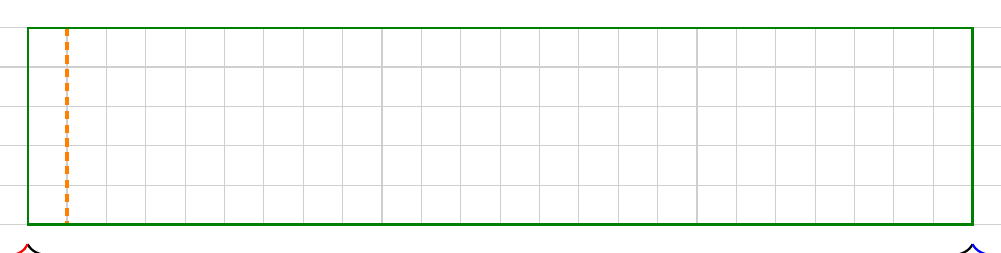
\begin{tikzpicture}
	\useasboundingbox (0,0) rectangle ({0.5*24},{-0.5*5}) ;
	\draw[xstep=0.5,ystep=0.5,thin,lightgray!75] ({-0.5*2},0) grid ({0.5*24+0.5*3},{-0.5*5}) ;
	\draw[thick,decorate,decoration={brace,amplitude=8pt,mirror}](0,{-0.5*5-0.25})--({0.5*24},{-0.5*5-0.25}) node[midway,below=8pt,font=\small\sffamily] {24C} ;
	\draw[red,thick,decorate,decoration={brace,amplitude=8pt,mirror}] ({-2*0.5},{-0.5*5-0.25})--({0},{-0.5*5-0.25}) node[midway,below=8pt,font=\small\sffamily] {2C} ;
	\draw[blue,thick,decorate,decoration={brace,amplitude=8pt,mirror}] ({0.5*24},{-0.5*5-0.25})--({0.5*24+3*0.5},{-0.5*5-0.25}) node[midway,below=8pt,font=\small\sffamily] {3C} ;
	\draw[thick,decorate,decoration={brace,amplitude=8pt}] ({0.5*24+3*0.5+0.25},0)--({0.5*24+3*0.5+0.25},{-0.5*5}) node[midway,right=8pt,font=\small\sffamily] {5C} ;
	\draw[very thick,orange,densely dashed] ({0.5*1},0)--({0.5*1},{-0.5*5}) ;
	\draw[green!50!black,thick] (0,0) rectangle ({0.5*24},{-0.5*5}) ;
\end{tikzpicture}

\vspace{1.25cm}

The \texttt{tikzpicture} is \textit{bounded} by the \textcolor{green!50!black}{\textit{border}}, in order to specify overtakings or alignment.

\smallskip

Le left-border of the \textcolor{green!50!black}{\textit{border}} is aligned on the left-margin of the page, so take care of the \texttt{\textbackslash parindent}.

\subsection{Predefined colors}

The package \textsf{WriteOnGrid} proposes "shortcuts" for classic colors !

\begin{PresentationCode}{listing only}
\definecolor{TyrianPurple}{rgb}{0.4,0.01,0.24}
\definecolor{PapierRose}{HTML}{E6B8E6}
\definecolor{PapierGris}{HTML}{D7E2EE}
%Colors for Seyes
\def\ColSeyes{PapierRose/PapierGris}
%Colors for Ruled
\def\ColRuled{PapierGris/TyrianPurple}
\end{PresentationCode}

\begin{PresentationCode}{text only}
{\tikz \filldraw[TyrianPurple] (0,0) rectangle++ (6,1) node[midway,font=\bfseries\large,text=white] {\verb+TyrianPurple+};}

{\tikz \filldraw[PapierRose] (0,0) rectangle++ (6,1) node[midway,font=\bfseries\large,text=black] {\verb+PapierRose+};}

{\tikz \filldraw[PapierGris] (0,0) rectangle++ (6,1) node[midway,font=\bfseries\large,text=black] {\verb+PapierGris+};}
\end{PresentationCode}

\subsection{The number of squares}

The number of grid squares (for individual grids and environments) can be given in several ways:

\begin{itemize}
	\item \Cle{NumSquares=<nbcols>x<nblines>} to specify manually;
	\item \Cle{NumSquares=Auto} to fill the rest of the page (horiz. and vert.);
	\item \Cle{NumSquares=Cx<nblines} to fill horizontally and specify the number of lines;
	\item \Cle{NumSquares=<nbcols>xL} to fill vertically and specify the number of columns.
\end{itemize}

Note that the calculations carried out to determine the remaining \textit{space} do not take into account any elastic springs that \LaTeX\ can add to \textit{optimize} the space.

\smallskip

To \textit{force} the addition of additional line(s), it is possible to use:

\begin{itemize}
	\item \Cle{NumSquares=Auto*} to force the addition of one more line;
	\item \Cle{NumSquares=Auto**} to force the addition of two more lines;
	\item \Cle{NumSquares=Auto***} to force the addition of three more lines;
	\item etc.
\end{itemize}

\pagebreak

\section{Commands, keys and options}

\subsection{The command}

\begin{PresentationCode}{listing only}
%command, with keys to prepare the grid

\DispGrid[keys]<color>
\end{PresentationCode}

The first argument, \textit{optional}, between \texttt{[...]} give the \Cle{keys} :

\begin{itemize}
	\item \Cle{NumSquares} to specify the size of the grid, under \texttt{(nbCol)x(nbRow)} ; \hfill~default : \Cle{17x5}
	\item \Cle{Unit} to specify the scale of the grid ; \hfill~default : \Cle{1}
	\item \Cle{Margin} to specify the global \textcolor{orange}{margin} at the beginning of the lines ; \hfill~default : \Cle{0}
	\item the boolean \Cle{DispBar} to display or not the bar ; \hfill~défaut : \Cle{true}
	\item \Cle{Enlarge} to specify the squares-overtakings, globally with \texttt{\textcolor{red}{L}\textcolor{blue}{R}} or side by side with \texttt{\textcolor{red}{L}/\textcolor{blue}{R}} ;\hfill~default : \Cle{0}
	\item the boolean \Cle{Border} to display the basis border of the grid ;\hfill~default : \Cle{false}
	\item the key\Cle{Grille}, from \Cle{5x5/Seyes/Ruled}, to specify the grid's type.\hfill~défaut : \Cle{5x5}
\end{itemize}

The second argument, \textit{optional}, between \texttt{<...>} is the color(s) of the grid :

\begin{itemize}
	\item by \Cle{Color} (\Cle{lightgray!50} by default) for $5\times5$  ;
	\item by \Cle{ColorA/ColorB} (\Cle{lightgray!50/lightgray!25} by default) for Seyes or Ruled.
\end{itemize}

\medskip

\begin{PresentationCode}{listing only}
%18x4 big squares, w/o overtaking, Seyes colors, w/o margin/bar
\DispGrid[NumSquares=18x4,Grid=Seyes,DispBar=false]<\ColSeyes>

%36x8 small squares, overtakings 3/3, PapierGris color
\DispGrid[NumSquares=36x8,Enlarge=3/3]<PapierGris>

%12x3 lines "Ruled", w/o overtakins, Ruled colors, centered, with 2-margin
\begin{center}
	\DispGrid[NumSquares=12x3,Grid=Ruled,Margin=2]<\ColRuled>
\end{center}
\end{PresentationCode}

\medskip

\DispGrid[NumSquares=18x4,Grid=Seyes,DispBar=false]<\ColSeyes>

\medskip

\DispGrid[NumSquares=36x8,Enlarge=3/3]<PapierGris>

\smallskip

\begin{center}
	\DispGrid[NumSquares=12x3,Grid=Ruled,Margin=2]<\ColRuled>
\end{center}

\pagebreak

\subsection{The environment}

\begin{PresentationCode}{listing only}
%environment, with keys to prepare the grid

\begin{EnvGrid}[keys]<color>
	...
\end{EnvGrid}
\end{PresentationCode}

The first argument, \textit{optional}, between \texttt{[...]} give the \Cle{keys} :

\begin{itemize}
	\item \Cle{NumSquares} to specify the size of the grid, under \texttt{(nbCol)x(nbRow)} ; \hfill~default : \Cle{17x5}
	\item \Cle{Unit} to specify the scale of the grid ; \hfill~default : \Cle{1}
	\item \Cle{Margin} to specify the global \textcolor{orange}{margin} at the beginning of the lines ; \hfill~default : \Cle{0}
	\item the boolean \Cle{DispBar} to display or not the bar ; \hfill~défaut : \Cle{true}
	\item \Cle{Enlarge} to specify the squares-overtakings, globally with \texttt{\textcolor{red}{L}\textcolor{blue}{R}} or side by side with \texttt{\textcolor{red}{L}/\textcolor{blue}{R}} ;\hfill~default : \Cle{0}
	\item the boolean \Cle{Border} to display the basis border of the grid ;\hfill~default : \Cle{false}
	\item the key\Cle{Grille}, from \Cle{5x5/Seyes/Ruled}, to specify the grid's type.\hfill~défaut : \Cle{5x5}
\end{itemize}

The second argument, \textit{optional}, between \texttt{<...>} is the color(s) of the grid :

\begin{itemize}
	\item by \Cle{Color} (\Cle{lightgray!50} by default) for $5\times5$  ;
	\item by \Cle{ColorA/ColorB} (\Cle{lightgray!50/lightgray!25} by default) for Seyes or Ruled.
\end{itemize}

\medskip

\begin{PresentationCode}{listing only}
%18x4 big squares, w/o overtaking, Seyes colors, 3-margin
\begin{EnvGrid}[NumSquares=18x4,Grid=Seyes,Margin=3]<\ColSeyes>
\end{EnvGrid}

%36x8 small squares, overtakings 3/3, PapierGris color
\begin{EnvGrid}[NumSquares=36x8,Enlarge=3/3]<PapierGris>
\end{EnvGrid}

%12x3 lines "Ruled", w/o overtakins, Ruled colors, centered, with 2-margin
\begin{center}
	\begin{EnvGrid}[NumSquares=12x3,Grid=Ruled,Margin=2]<\ColRuled>
	\end{EnvGrid}
\end{center}
\end{PresentationCode}

\medskip

\begin{EnvGrid}[NumSquares=18x4,Grid=Seyes,Margin=3]<\ColSeyes>
\end{EnvGrid}

\smallskip

\begin{EnvGrid}[NumSquares=36x8,Enlarge=3/3]<PapierGris>
\end{EnvGrid}

\smallskip

\begin{center}
	\begin{EnvGrid}[NumSquares=12x3,Grid=Ruled,Margin=2]<\ColRuled>
	\end{EnvGrid}
\end{center}

\pagebreak

\subsection{Write on the lines}

The idea is to write on the created grid (environment !). In order to write \textit{right} on the lines, we can :

\begin{itemize}
	\item give the lines one by one ;
	\item avoid using multilines paragraps, items ;
	\item pass a line.
\end{itemize}

\begin{PresentationCode}{listing only}
...
	%to write the lines, one by one
	\WriteLine[keys]<alignment>{text}
	%to pass the ligne
	\PassLine
...
\end{PresentationCode}

The fisrt argument, \textit{optional}, between \texttt{[...]} give the \Cle{keys} :

\begin{itemize}
	\item \Cle{OffsetH}, in squares, to shift the text from the \textcolor{orange}{margin} ; \hfill~default : \Cle{0}
	\item \Cle{OffsetV} to shift vertically the line ; \hfill~default : \Cle{0pt}
	\item \Cle{Scale} to specify the scale of the given text.\hfill~default : \Cle{1}
\end{itemize}

the second argument, \textit{optional}, between \texttt{<...>} is the horizontal alignment (\Cle{left/center/right}) of the text in the basis \textcolor{green!50!black}{\textit{border}}, \Cle{left} by default.

\medskip

Le third argument, \textit{mandatory} and between \texttt{\{...\}} is the text, eventually with options.

\begin{PresentationCode}{listing only}
\begin{EnvGrid}[NumSquares=36x8]
	\WriteLine[Scale=1.5]{my text on ligne 1\ldots}
	\WriteLine[Scale=1.5]<center>{\ttfamily my tetetype text centered on line 2\ldots}
	\WriteLine[Scale=1.5]<right>{right-align text on line 3\ldots}
	\WriteLine[Scale=1.5,OffsetH=0.1]{\textcolor{red}{red text, 1mm-shifted\ldots}}
	\PassLine
	\WriteLine[Scale=0.5]{\sffamily sans serif text, reduced by 50\,\%, on line 6\ldots}
	\WriteLine[Scale=1.5,OffsetH=3]{\cursive 3 squares-shifted text\ldots}
\end{EnvGrid}
\end{PresentationCode}

\begin{EnvGrid}[NumSquares=36x8]
	\WriteLine[Scale=1.5]{my text on ligne 1\ldots}
	\WriteLine[Scale=1.5]<center>{\ttfamily my tetetype text centered on line 2\ldots}
	\WriteLine[Scale=1.5]<right>{right-align text on line 3\ldots}
	\WriteLine[Scale=1.5,OffsetH=0.1]{\textcolor{red}{red text, 1mm-shifted\ldots}}
	\PassLine
	\WriteLine[Scale=0.5]{\sffamily sans serif text, reduced by 50\,\%, on line 6\ldots}
	\WriteLine[Scale=1.5,OffsetH=3]{\cursive 3 squares-shifted text\ldots}
\end{EnvGrid}

\begin{PresentationCode}{listing only}
\begin{EnvGrid}[NumSquares=16x4,Margin=2,Grid=Ruled]<\ColRuled>
	\WriteLine[Scale=1.5]{\textcolor{red}{red text on line 1\ldots}}
	\WriteLine[Scale=1.15,OffsetH=1]{$(1+x)^2=1+2x+x^2$ on line 2, with 1-square offset\ldots}
	\WriteLine[OffsetH=-1]{\textcolor{blue}{blue text, back to left, on line 3\ldots}}
\end{EnvGrid}

\end{PresentationCode}
\begin{EnvGrid}[NumSquares=16x4,Margin=2,Grid=Ruled]<\ColRuled>
	\WriteLine[Scale=1.5]{\textcolor{red}{red text on line 1\ldots}}
	\WriteLine[Scale=1.15,OffsetH=1]{$(1+x)^2=1+2x+x^2$ on line 2, with 1-square offset\ldots}
	\WriteLine[OffsetH=-1]{\textcolor{blue}{blue text, back to left, on line 3\ldots}}
\end{EnvGrid}

\newpage

\part*{Additional informations}

\section{Introduction}

There's few other possibilities with the package\textsf{WorkOnGrid}, but for the moment only with \textit{french} keys, so there's no specific documentation for these commands.

\smallskip

To sum up, they create full paper grid (by preference for \texttt{\textbf{a4paper}}), with the ability to write paragraph.

\section{Example}

\begin{PresentationCode}{listing only}
\begin{PleinePageRuled}[NumLignes]
	\LignePapierRuled[Echelle=1.25,Ligne=1]{C. PIERQUET \hfill LaTeX}
	\LignePapierRuled[Echelle=1.25,Ligne=2,Couleur=red]<center>{\underline{\cursive\bfseries Evaluation 3}}
	\CadreNoteRuled{3}
	\LignePapierRuled[Echelle=1.25,Ligne=8,Couleur=green!50!black]{\sffamily\underline{Exercise 1 :}}
	\ParagraphePapierRuled[Ligne=9]{\cursive\lipsum[1]}
	\ParagraphePapierRuled[Ligne=22]
	{%
		We try with math, $1+\frac12=\frac32$, inline, with several lines.\\
		And another math example, $\int_0^1 2x dx = 1$.\\
		A new line now !
	}
\end{PleinePageRuled}
\end{PresentationCode}

\pagebreak

\thispagestyle{empty}

\begin{PleinePageRuled}
	\LignePapierRuled[Echelle=1.25,Ligne=1]{C. PIERQUET \hfill LaTeX}
	\LignePapierRuled[Echelle=1.25,Ligne=2,Couleur=red]<center>{\underline{\cursive\bfseries Evaluation 3}}
	\CadreNoteRuled{3}
	\LignePapierRuled[Echelle=1.25,Ligne=8,Couleur=green!50!black]{\sffamily\underline{Exercise 1 :}}
	\ParagraphePapierRuled[Ligne=9]{\cursive\lipsum[1]}
	\ParagraphePapierRuled[Ligne=22]
	{%
		We try with math, $1+\frac12=\frac32$, inline, with several lines.\\
		And another math example, $\int_0^1 2x dx = 1$.\\
		A new line now !
	}
\end{PleinePageRuled}

\pagebreak

\part*{History}

\verb|v0.1.7|~:~~~~New feature for french paper \textsf{PleinePageCinqCinq}

\verb|v0.1.6|~:~~~~Possibility to automatically determine L\&C based on the remaining space.

\verb|v0.1.4|~:~~~~New \texttt{[keys]} + enhancements for paragraphs, for french version (for the moment\dots)

\verb|v0.1.4|~:~~~~\texttt{xcolor} isn't loaded with \textsf{[table,svgnames]})

\verb|v0.1.3|~:~~~~Command to display a grid (w/o writing on it)

\verb|v0.1.2|~:~~~~Shortcuts for default colors + small bugfixes

\verb|v0.1.1|~:~~~~Best color choice

\verb|v0.1.0|~:~~~~Initial version

\end{document}